\noindent
{\bf 3. Partitioning a Path}
\medskip

In this section we present an optimal algorithm to perform
parametric search on a path of $n$ vertices.
The first phase gathers information with which subsequent feasibility tests
can be performed in $o(n)$ time.
The second phase then completes the parametric search using this
faster feasibility testing.
Our discussion focuses on the max-min problem;
at the end of the section we identify the changes necessary
for the min-max problem.
Throughout this section we assume that the vertices of any path or subpath
are indexed in increasing order from the start to the end of the path.

We first consider the running time of {\it PATH0},
to determine how the approach might be accelerated.
All activities except for feasibility testing use a total of $O(n)$ time.
Feasibility testing uses $\Theta (n \log n)$ time in the worst case,
since there will be $\Theta (\log n)$ values to be tested in the worst case,
and the test takes $\Theta (n)$ time.
It seems unlikely that one can reduce the number of tests that need to be made,
so that to design a linear-time algorithm,
it seems necessary to design a feasibility test that takes $o(n)$ time.
We show how to realize such an approach.

We shall represent the path by a partition into subpaths,
each of which can be searched in time proportional to the
logarithm of its length.
Each such subpath will possess a property
that makes feasibility testing easier.
Either the subpath will be singular or stable.
A subpath $P'$ is {\it singular} if it consists of one vertex,
and it is {\it stable} if no value in $M(P')$ falls in the interval
$(\lambda_1, \lambda_2 )$.
If a subpath is stable,
then the position of any one cut determines the positions
of all other cuts in the subpath,
irrespective of what value of $\lambda$ is chosen from within
$(\lambda_1, \lambda_2 )$.
If suitable data structures are set up when the stable subpath
is added to the partition of $P$,
then a linear scan of the subpath is not needed.

To make the representation simple,
the subpaths in the partition are restricted to have lengths
that are powers of 2.
Each subpath will consist of vertices whose indices are
$(j-1)2^i+1, \ldots ,j\:2^i$ for integers $j>0$ and $i \geq 0$.
Initially the partition will consist of $n$ singular subpaths.
Each nonsingular subpath will have $i>0$.
When introduced into the partition,
it will replace its two {\it constituent subpaths},
the first with indices $(2j-2)2^{i-1}+1, \ldots ,(2j-1)2^{i-1}$,
and the second with indices $(2j-1)2^{i-1}+1, \ldots ,(2j)2^{i-1}$.

The partition of path $P$ into the subpaths can be represented
using three arrays $last[1..n]$, $ncut[1..n]$ and $next[1..n]$.
Consider any subpath in the partition,
with first vertex $v_f$ and last vertex $v_t$.
Let $v_l$ be an arbitrary vertex in the subpath.
The array $last$ identifies the end of a subpath,
given the first vertex of a subpath.
Thus $last(l)=t$ if $l=f$ and is arbitrary otherwise.
Given a cut on the subpath,
the array $next$ identifies,
in constant time, a cut further on in that subpath.
The array $ncut$ identifies the number of cuts skipped
in moving to that further cut.
Let $w(l,t)$ be the sum of the weights of vertices $v_l$ through $v_t$.
If $w(l,t) < \lambda_2$,
then $next(l)=0$ and $ncut(l)=0$.
Otherwise, $next(l) \geq l$ is the index of the last vertex before a cut,
given that $l=1$ or $v_l$ is the first vertex after a cut.
Then $ncut(l)$ is the number of cuts after $v_l$ up to and including the one
following $v_{next(l)}$.
We assume that the last cut on a subpath will leave
a (possibly empty) subset of vertices of total weight less than $\lambda_2$.
(Note that the last cut on the path as a whole must then be ignored.)

Given the partition into subpaths, we describe feasibility test {\it FTEST1}.
Let $\lambda$ be the value to be tested,
with $\lambda_1 < \lambda < \lambda_2$.
For each subpath, we use binary search to find the first cut,
and then, follow $next$ pointers and add $ncut$ values to
identify the number of cuts on the subpath.
When we follow a path of $next$ pointers,
we will compress this path.
This turns out to be a key operation as we consider
subpath merging and its effect on feasibility testing.
(Note that the path compression makes
{\it FTEST1} a function with side effects.)\\

\sspace
\noindent
{\bf func} {\it FTEST1} ({\bf path} $P$, {\bf integer} $k$, {\bf real} $\lambda$){\vspace{.05in}\\
$\T $ $f \ASG 1$\\
$\T $ $numcut \ASG -1$; $remainder\ASG 0$\\
$\T $ $\WH$ $f \leq n$ $\DO$ /* search the next subpath: */\\
$\T \T $ $t \ASG last(f)$\\
$\T \T $ $\IF$ $remainder + w(f,t) < \lambda$\\
$\T \T $ $\TN$ $remainder \ASG remainder + w(f,t)$\\
$\T \T $ $\EL$ \\
$\T \T \T $ $numcut \ASG numcut+1$ \\
$\T \T \T $ Binary search for the smallest $r$ such that $w(f,r) + remainder \geq \lambda$. \\
$\T \T \T $ $\IF$ $r<t$ \\
$\T \T \T $ $\TN$ \\
$\T \T \T \T $ $(s,sumcut) \ASG$ {\it search\_next\_path} $(r,t)$\\
$\T \T \T \T $ $numcut \ASG numcut+sumcut$ \\
$\T \T \T \T $ {\it compress\_next\_path} $(r,s,t,sumcut)$ \\
$\T \T \T $ $\EI$  \\
$\T \T \T $ $remainder \ASG w(s+1,t)$ \\
$\T \T $ $\EI$  \\
$\T \T $ $f \ASG t+1$  \\
$\T $ $\EW$ \\
$\T $ $\IF$ $numcut \geq k$ $\TN$ {\bf return}(``$lower$'') $\EL$ {\bf return}(``$upper$'') $\EI$ \\
{\bf endfunc}
 
\bigskip
\noindent
{\it search\_next\_path} ({\bf vertex\_index} $l,t$)\vspace{.05in}\\
$\T $ $sumcut \ASG 0$ \\
$\T $ $\WH$ $l < t$ and $next(l+1) \neq 0$ \\
$\T \T $ $sumcut \ASG sumcut+ncut(l+1)$ \\
$\T \T $ $l \ASG next(l+1)$ \\
$\T $ $\EW$ \\
$\T $ {\bf return}$((l,sumcut))$ 
 
\bigskip
\noindent
{\it compress\_next\_path} ({\bf vertex\_index} $l,s,t$, {\bf integer} $sumcut$)\vspace{.05in}\\
$\T $ $\WH$ $l < t$ and $next(l+1) \neq 0$ \\
$\T \T $ $sumcut \ASG sumcut-ncut(l+1)$ \\
$\T \T $ $ncut(l+1) \ASG ncut(l+1)+sumcut$ \\
$\T \T $ $temp \ASG next(l+1)$ \\
$\T \T $ $next(l+1) \ASG s$ \\
$\T \T $ $l \ASG temp$ \\
$\T $ $\EW$  

\dspace
\bigskip

Use of this feasibility test is alone not enough to guarantee
a reduction in the time for feasibility testing.
This is because there is no assurance that the interval
$(\lambda_1, \lambda_2)$ will be narrowed in a manner
that allows longer subpaths to quickly replace shorter subpaths
in the partition of path $P$.
To achieve this effect,
we reorganize the positive values from $M(P)$
into submatrices that correspond in a natural way to subpaths.
Furthermore, we associate weights with these submatrices
and use these weights in selecting the weighted median for testing.
The weights will place a premium on resolving first
the values from submatrices corresponding to short subpaths.
However, using weights could mean that many values of small weight
could be considered repeatedly,
causing the total time for selection to exceed $\Theta (n)$.
To offset this effect, we also find the unweighted median,
and test this value.
This approach guarantees that at least half of the submatrices'
representatives are discarded on each iteration,
so that each submatrix inserted into $\cal M$ need be charged
only a constant for its share of the total work in
selecting values to test.

We now proceed to a broad description of {\it PATH1}.
The basic structure follows that of {\it PAR\_SEARCH},
in that there will be the routines
{\it PATH1\_init\_mat},
{\it PATH1\_test\_val},
and {\it PATH1\_update\_mat}.
However, we will slip the set-up and manipulation
of the data structures for the subpaths into the routines
{\it PATH1\_init\_mat} and {\it PATH1\_update\_mat}.
Let $large(M)$ be the largest element in submatrix $M$,
and let $small(M)$ be the smallest element in $M$.\\
 
\sspace
\noindent
{\it PATH1\_init\_mat}:\vspace{.05in}\\
$\T $ Initialize $\cal M$ to be empty. \\
$\T $ Call {\it mats\_for\_path}$(P,1,n)$ to insert submatrices of $M(P)$ into $\cal M$. \\
$\T $ $\FO$ $l \ASG 1$ $\TO$ $n$ $\DO$ $last(l) \ASG l$; $next(l) \ASG 0$; $ncut(l) \ASG 0$ $\EF$
 
\bigskip
\noindent
{\it PATH1\_test\_val}:\vspace{.05in}\\
$\T $ $R \ASG \emptyset$ \\
$\T $ $\FO$ each $M$ in $\cal M$ $\DO$ \\
$\T \T $ $\IF$ $large(M) < \lambda_2$ $\TN$ Insert $large(M)$ into $R$ with weight $w(M)/4$. $\EI$ \\
$\T \T $ $\IF$ $small(M) > \lambda_1$ $\TN$ Insert $small(M)$ into $R$ with weight $w(M)/4$. $\EI$ \\
$\T $ $\EF$ \\
$\T$ Select the weighted median element $\lambda$ in $R$. \\
$\T$ $\IF$ {\it FTEST1}$(P,k,\lambda ) = ``lower$'' $\TN$ $\lambda_1 \ASG \lambda$ $\EL$ $\lambda_2 \ASG \lambda$ $\EI$ \\
$\T$ Remove from $R$ any values no longer in $(\lambda_1,\lambda_2)$. \\
$\T$ $\IF$ $R$ is not empty \\
$\T$ $\TN$ \\
$\T \T$ Select the unweighted median element $\lambda '$ in $R$. \\
$\T \T$ $\IF$ {\it FTEST1}$(P,k,\lambda ') = ``lower$'' $\TN$ $\lambda_1 \ASG \lambda '$ $\EL$ $\lambda_2 \ASG \lambda '$ $\EI$ \\
$\T$ $\EI$ 
 
\bigskip
\noindent
{\it PATH1\_update\_mat}:\vspace{.05in}\\
$\T $ $\WH$ there is an $M$ in $\cal M$ such that $small(M) \geq \lambda_2$ or $large(M) \leq \lambda_1$ \\
$\T \T $ or $small(M) \leq \lambda_1 \leq \lambda_2 \leq large(M)$ $\DO$ \\
$\T \T $ $\IF$ $small(M) \geq \lambda_2$ or $large(M) \leq \lambda_1$ \\
$\T \T $ $\TN$ \\
$\T \T \T $ Delete $M$ from $\cal M$. \\
$\T \T \T $ $\IF$ this is the last submatrix remaining for a subpath $P'$ \\
$\T \T \T $ $\TN$ $glue\_paths(P')$ \\
$\T \T \T $ $\EI$ \\
$\T \T $ $\EI$ \\
$\T \T $ $\IF$ $small(M) \leq \lambda_1$ and $large(M) \geq \lambda_2$ \\
$\T \T $ $\TN$ Split $M$ into four square submatrices, each of weight $w(M)/8$. \\
$\T \T $ $\EI$ \\
$\T $ $\EW$
 
\dspace
\bigskip

\begin{figure}[thb]
\begin {center}
%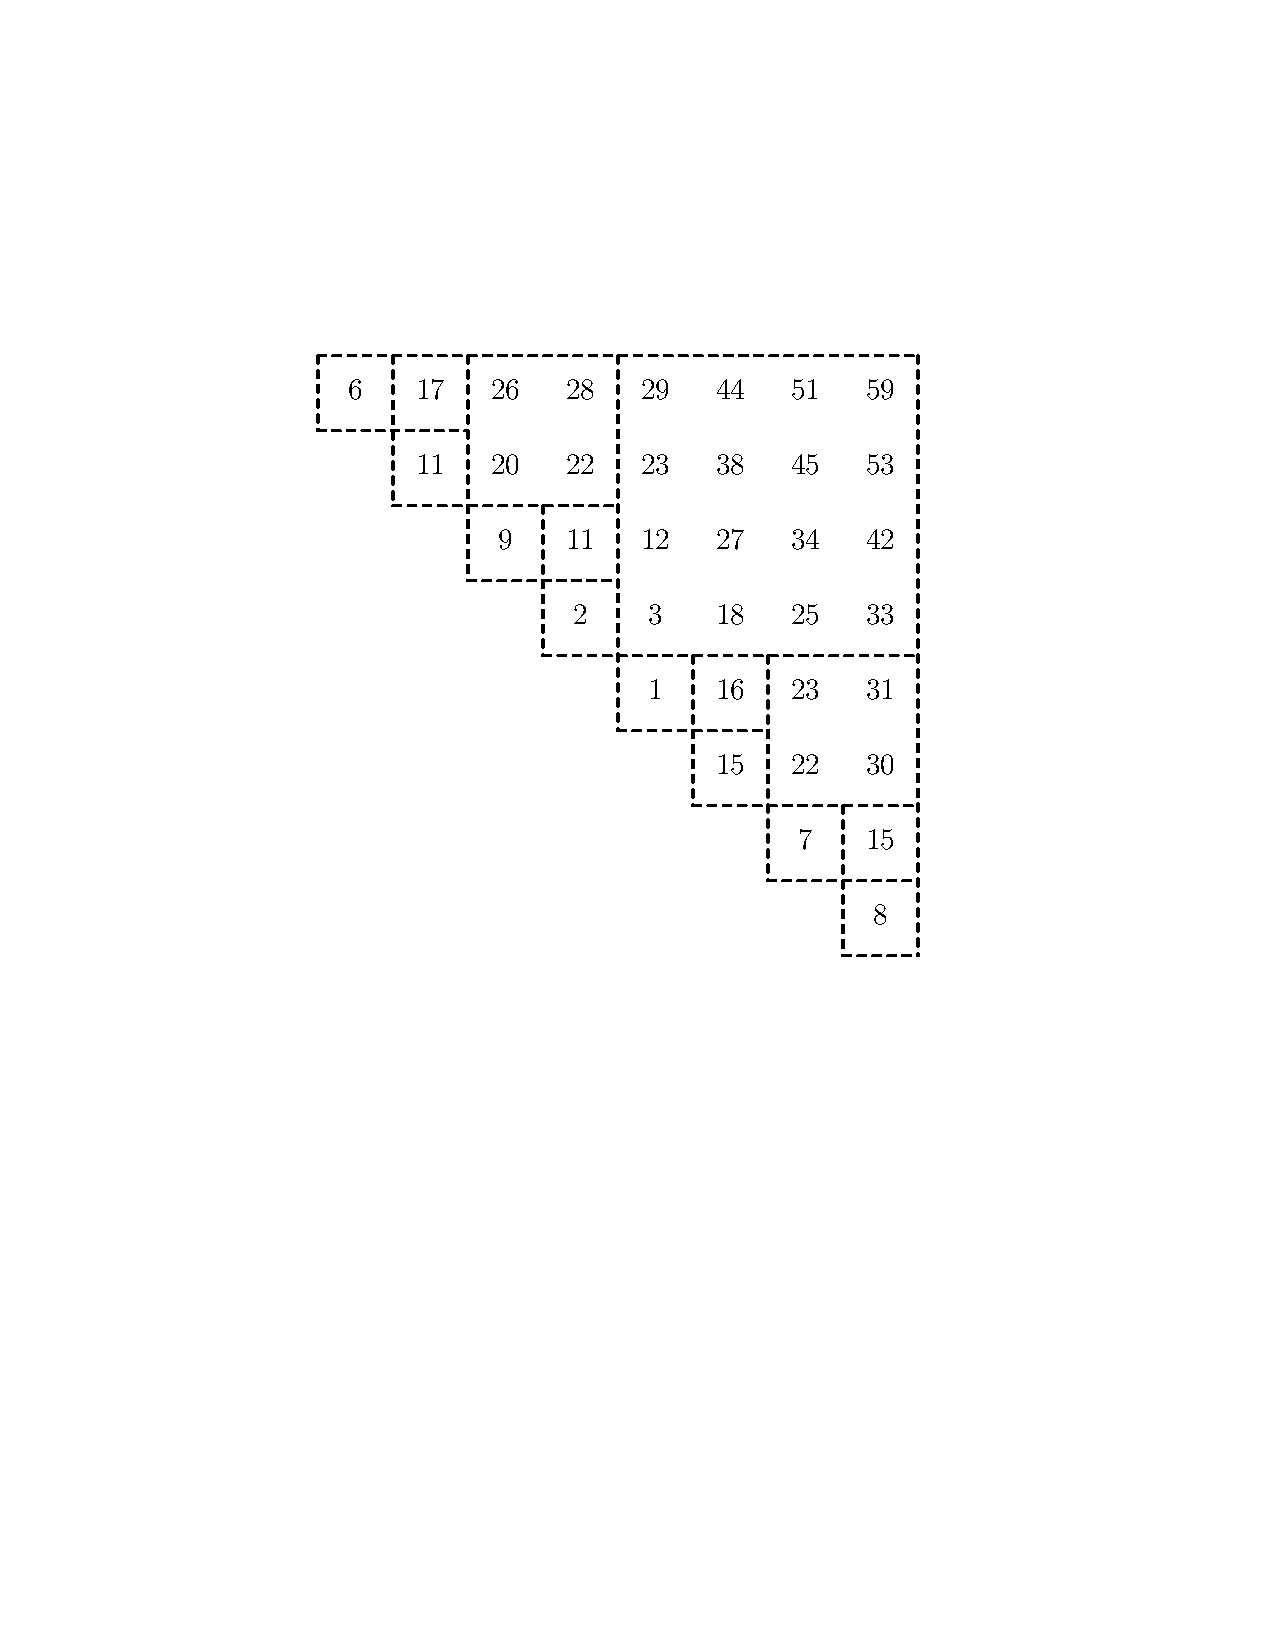
\includegraphics{fig3p1.epsi}
\end{center}
{\caption{\small Initial submatrices for $M(P)$ in {\it PATH1}}\label{fig3p1}}
\end{figure}

\begin{figure}[thb]
\begin {center}
%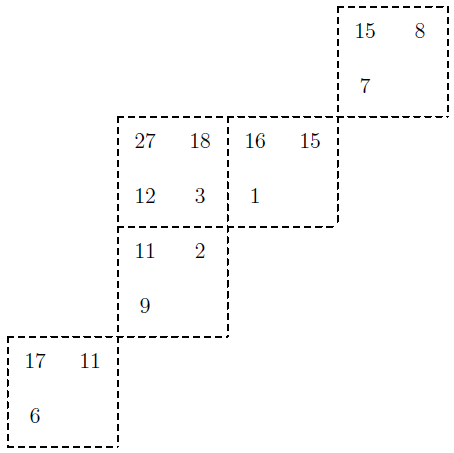
\includegraphics{fig3p2.epsi}
\end{center}
{\caption{\small TO BE FILLED IN??}\label{fig3p2}}
\end{figure}

Below is the procedure {\it mats\_for\_path},
which inserts submatrices of appropriate weight into $\cal M$.
A call with arguments $f$ and $t$
will generate submatrices for all required subpaths of
a path containing the vertices with indices $f,\ldots ,t$.
(In this section, we assume that $f=1$ and $t=n$,
but we state the procedure in this form so that it can be used
in the next section too.)
The submatrices for the matrix $M(P)$ in Fig.~\ref{fig2p1}
are shown in Fig.~\ref{fig3p1}. [REDO FOR NEW DEF]
Every subpath $P'$ that will appear in some partition of $P$
is initialized with $cleaned(P')$ and $glued(P')$ to {\bf false},
where $cleaned(P')$ indicates whether or not all values in
the submatrix associated with $P'$ are outside the interval
$(\lambda_1,\lambda_2)$ ,
and $glued(P')$ indicates whether or not all values in $M(P')$
are outside the interval $(\lambda_1,\lambda_2)$. \\

\sspace
\noindent
{\bf proc} {\it mats\_for\_path} ({\bf path} $P$, {\bf integer} $f,t$){\vspace{.05in}\\
$\T $ $size \ASG 1$ \\
$\T $ $w \ASG 4n^4$ \\
$\T $ $\WH$ $f\leq t$ $\DO$ \\
$\T \T $ $\FO$ $i \ASG f$ $\TO$ $t$ $\BY$ $size$ $\DO$ \\
$\T \T \T $ Insert submatrix $[i\:..\:(i\!+\!\lceil size/2\rceil\!-\!1), (i\!+\!\lceil size/2\rceil )..\:(i\!+\!size\!-\!1)]$ \\
$\T \T \T \T $of $M(P)$ into $\cal M$ with weight $w$. \\
$\T \T \T $ Let $P'$ be the subpath whose vertices have indices $i,\ldots ,i+size-1$. \\
$\T \T \T $ $cleaned(P') \ASG \FA$; $glued(P') \ASG \FA$ \\
$\T \T \T $ $\EF$ \\
$\T \T $ $size \ASG size*2$ \\
$\T \T $ $w \ASG w/2$ \\
$\T \T $ $f \ASG size*\lceil (f-1)/size\rceil +1$ \\
$\T \T $ $t \ASG size*\lfloor t/size\rfloor$ \\
$\T $ $\EW$  \\
{\bf endproc}\\

\dspace
\bigskip

We next describe the procedure {\it glue\_paths},
which checks to see if two constituent subpaths can be combined together.
To glue two subpaths $P_2$ and $P_3$ together into a subpath $P_1$,
we must have $(glued(P_2)$ {\bf and} $glued(P_3)$ {\bf and} $cleaned(P_1))$.
Let $P'$ be any subpath of weight at least $\lambda_2$,
and let $f'$ and $t'$ be the indices of the first and last vertices in $P'$,
resp.
Let the $\lambda$-{\it prefix} of $P'$, designated $\lambda${\it pref}$\,(P')$,
be vertices $v_{f'},\cdots ,v_l$ in $P'$ where $l$ is the largest index
such that $w(f',l) < \lambda_2$.
Let the $\lambda$-{\it suffix} of $P'$, designated $\lambda${\it suff}$\,(P')$,
be vertices $v_l,\cdots ,v_{t'}$ in $P'$ where $l$ is the smallest index
such that $w(l,t') < \lambda_2$.
Procedure {\it glue\_paths} sets the $next$ pointers from
vertices in $\lambda${\it suff}$\,(P_2)$ to vertices
in $\lambda${\it pref}$\,(P_3)$. \\

\sspace
\noindent
{\bf proc} {\it glue\_paths} ({\bf path} $P_1$){\vspace{.05in}\\
$\T $ $cleaned(P_1) \ASG \TR$\\
$\T $ $\IF$ $P_1$ has length 1\\
$\T $ $\TN$ \\
$\T \T $ $glued(P_1) \ASG \TR$ \\
$\T \T $ Let $l$ be the index of the vertex in $P_1$. \\
$\T \T $ $\IF$ $w(l,l) \geq \lambda_2$ $\TN$ $next(l) \ASG l$; $ncut(l) \ASG 1$ $\EI$ \\
$\T \T $ Reset $P_1$ to be the subpath of which $P_1$ is now a constituent subpath. \\
$\T $ $\EI$ \\
$\T $ Let $P_2$ and $P_3$ be the constituent subpaths of $P_1$. \\
$\T $ $\WH$ $glued(P_2)$ and $glued(P_3)$ and $cleaned(P_1)$ and $P_1 \neq P$ $\DO$ \\
$\T \T $ $glued(P_1) \ASG \TR$\\
$\T \T $ Let $f_2$ and $t_2$ be resp. the indices of the first and last vertices in $P_2$. \\
$\T \T $ Let $f_3$ and $t_3$ be resp. the indices of the first and last vertices in $P_3$. \\
$\T \T $ $last(f_2) \ASG t_3$\\
$\T \T $ $\IF$ $w(f_2,t_3) \geq \lambda_2$\\
$\T \T $ $\TN$ \\
$\T \T \T $ $\IF$ $w(f_2,t_2) < \lambda_2$ \\
$\T \T \T $ $\TN$ $f \ASG f_2$ \\
$\T \T \T $ $\EL$ /* initialize $f$ to the front of $\lambda${\it suff}$\,(P_2)$ */ \\
$\T \T \T \T $ $f \ASG t_2$\\
$\T \T \T \T $ $\WH$ $w(f-1,t_2) < \lambda_2$ $\DO$ $f \ASG f-1$ $\EW$ \\
$\T \T \T $ $\EI$ \\
$\T \T \T $ $t \ASG f_3$ \\
$\T \T \T $ $\WH$ $f \leq t_2$ and $w(f,t_3) \geq \lambda_2$ $\DO$ /* set $next$ pointers for $\lambda${\it suff}$\,(P_2)$ */ \\
$\T \T \T \T $ $\WH$ $w(f,t) < \lambda_2$ $\DO$ $t \ASG t+1$ $\EW$ \\
$\T \T \T \T $ $ncut(f) \ASG 1$ \\
$\T \T \T \T $ $next(f) \ASG t$ \\
$\T \T \T \T $ $f \ASG f+1$ \\
$\T \T \T $ $\EW$ \\
$\T \T $ $\EI$  \\
$\T \T $ Reset $P_1$ to be the subpath of which $P_1$ is now a constituent subpath. \\
$\T \T $ Let $P_2$ and $P_3$ be the constituent subpaths of $P_1$. \\
$\T $ $\EW$ \\
{\bf endproc}\\

\dspace

It would nice if procedure {\it glue\_paths},
after setting pointers in $\lambda${\it suff}$\,(P_2)$,
would perform pointer jumping,
so that $next$ pointers for vertices in $\lambda${\it pref}$\,(P_1)$
would point to vertices in $\lambda${\it suff}$\,(P_1)$.
Unfortunately, it appears that requiring {\it glue\_paths}
to perform such an activity would result in a total time
over all calls of $O(n \log \log n)$ in the worst case.
(We do not have a proof of this assertion,
but extensive simulation seems to provide strong corroboration
for such a conjecture.)
We opt for having {\it glue\_paths} do no pointer jumping,
and instead we do pointer jumping under the guise of path
compression in {\it FTEST1}.
We use an argument based on amortization to show that this works well.
\bigskip

\noindent
{\bf Lemma 3.1.}
Let $P$ be a path of $n$ vertices.
All calls to {\it glue-paths} will take amortized time of $O(n)$,
and {\it FTEST1} will search each subpath 
in amortized time proportional to the logarithm of its length.

\noindent
{\bf Proof.}
Suppose two subpaths $P_2$ and $P_3$ are glued together to give $P_1$,
where $P_1$ has weight at least $\lambda_2$.
We consider two cases.
First suppose either $P_2$ or $P_3$ has weight at most $\lambda_1$.
Let $P_m$ represent this subpath.
The time for {\it glue\_paths} is in worst case proportional
to the length of $P_m$.
Also, we leave a {\it glue-credit}
on each vertex in the $\lambda${\it pref}$\,(P_1)$ and $\lambda${\it suff}$\,(P_1)$,
and a {\it jump-credit} on each vertex in the $\lambda${\it pref}$\,(P_1)$.
The number of credits will be proportional to the length of $P_m$.
We charge this work and the credits to the vertices of $P_m$,
at a constant charge per vertex.
It is clear that any vertex in $P$ is charged at most once,
so that the total charge to vertices over all calls to {\it glue\_paths}
is $O(n)$.
The second case is when both $P_2$ and $P_3$ have weight at least $\lambda_2$.
In this case, the time for {\it glue\_paths} is proportional to the sum
of the lengths of $\lambda${\it suff}$\,(P_2)$
and $\lambda${\it pref}$\,(P_3)$,
and we use the glue-credits of $P_2$ and $P_3$ to pay for this.
The jump-credits are used by {\it FTEST1} rather than {\it glue-paths},
but we discuss below how they might have been used by {\it glue-paths}.

Suppose both $P_2$ and $P_3$ have weight at least $\lambda_2$.
Then we might have wanted to have {\it glue-paths} jump the $next$ pointers
so that the $next$ pointer for a vertex in $\lambda${\it pref}$\,(P_2)$
will be reset to point to $\lambda${\it suff}$\,(P_3)$.
The time to reset such pointers will be proportional to the length
of $\lambda${\it pref}$\,(P_2)$.
The jump-credits of $\lambda${\it pref}$\,(P_3)$ could pay for this,
as long as the length of $\lambda${\it pref}$\,(P_2)$
is at most some constant (say 2)
times the length of the $\lambda${\it pref}$\,(P_3)$.
When the length of the $\lambda${\it pref}$\,(P_2)$
is at most twice the length of the $\lambda${\it pref}$\,(P_3)$,
we would not want to jump the pointers.

In general we could view a subpath as containing a sequence of
$\lambda$-{\it regions},
where each $\lambda$-region was once the $\lambda$-prefix of some subpath,
and the length of a $\lambda$-region is less than twice the length
of the preceding $\lambda$-region.
Note that the number of $\lambda$-regions in the sequence could be at most
the logarithm of the length of the subpath.
When gluing two subpaths together,
we could concatenate their sequences of $\lambda$-regions together,
and jump pointers over any $\lambda$-region that gets a predecessor
whose length is not more than twice its length.
Its jump-credits could then be used for this pointer jumping.
Searching a subpath in {\it FTEST1} would then take
time at most proportional to its length.

Of course {\it glue-paths} does not jump pointers.
However,
a lazy form of pointer-jumping is found in the path-compression of {\it FTEST1},
and the same sort of analysis can be seen to apply.
Suppose that {\it FTEST1} follows a pointer to a vertex
that was once in the $\lambda$-prefix of some subpath.
Consider the situation if {\it glue-paths} had jumped pointers.
If that pointer would have been present in the sequence of $\lambda$-regions,
then charge the operation of following that pointer to {\it FTEST1}.
Otherwise, charge the operation of following that pointer
to the jump-credits of the $\lambda$-prefix containing the vertex.
It follows that the number of pointers followed during a search
of a subpath that are not covered by jump-credits is at most
the logarithm of the length of the subpath.
Also, the binary search to find the position of the first cut
on a subpath uses time at most proportional
to the logarithm of the length of the subpath.
$\Box$

\bigskip

\noindent
{\bf Lemma 3.2.}
Let $P$ be a path of $n$ vertices.
On the $i$-th iteration of the while-loop of {\it PATH1},
the amortized time used by feasibility test {\it FTEST1}
will be $O(i(5/6)^{i/5}\:n)$.

\noindent
{\bf Proof.}
We first consider the weights assigned to submatrices in $\cal M$.
Corresponding to subpaths of lengths $1, 2, 4, \ldots , n$,
procedure {\it mats\_for\_path} creates
$n$ submatrices of size $1 \times 1$,
$n/2$ submatrices of size $1 \times 1$,
$n/4$ submatrices of size $2 \times 2$, and so on,
up through one submatrix of size $n/2 \times n/2$.
The total weight of the submatrices corresponding to each path length is
$4n^5, n^5, n^5/4, \ldots , 4n^3$, resp.
It follows that the total weight for submatrices of all path lengths is
less than $(4/3)*4n^5$.

Let $wgt(M)$ be the weight assigned to submatrix $M$.
Define the {\it effective weight},
denoted {\it eff\_wgt}$(M)$, of a submatrix $M$ in $\cal M$
to be $wgt(M)$ if both its smallest value and largest value
are contained in the interval $(\lambda_1, \lambda_2)$
and $(3/4)wgt(M)$ if only one of its smallest value and largest value
is contained in the interval $(\lambda_1, \lambda_2)$.
Let {\it eff\_wgt}$(\cal M )$ be the total effective weight of all submatrices in $\cal M$.
When a feasibility test renders a value (the smallest or largest)
from $M$ no longer in the interval $(\lambda_1, \lambda_2)$,
we argue that {\it eff\_wgt}$(M)$ is reduced by at least $wgt(M)/4$
because of that value.
If both values were contained in the interval $(\lambda_1, \lambda_2)$,
and one is no longer is, then clearly it is true.
If only one value was contained in the interval $(\lambda_1, \lambda_2)$,
and it no longer is,
then $M$ is replaced by four submatrices of effective weights
$wgt(M)/8 + wgt(M)/8 + (3/4)wgt(M)/8 + (3/4)wgt(M)/8$ $< wgt(M)/2$,
so that there is a reduction in weight by greater than $wgt(M)/4$.
If both values were contained in the interval $(\lambda_1, \lambda_2)$,
and both are no longer in,
then we consider first one and then the other.
Thus every element that was in $(\lambda_1, \lambda_2)$ but no longer is
causes a decrease in {\it eff\_wgt}$(\cal M )$ by an amount
at least equal to its weight in $R$.
Values with at least half of the total weight in $R$
find themselves no longer in $(\lambda_1, \lambda_2)$.
Furthermore, the total weight of $R$ is at least $1/3$ of
{\it eff\_wgt}$(\cal M )$.
This follows since a submatrix $M$ has either two values in $R$
at a total of $2w(M)/4 = (1/2)w(M)$
or one value at a weight of $w(M)/4 = (1/3)(3w(M)/4)$.
Thus {\it eff\_wgt}$(\cal M )$
decreases by a factor of at least $(1/2)(1/3) = 1/6$ per iteration.

Corresponding to the subpaths of length $2^j$,
there are $n/2^j$ submatrices created by {\it mats\_for\_path}.
If such a matrix is quartered repeatedly until $1 \times 1$ submatrices result,
each such submatrix will have weight $n^4/2^{4j-5}$.
Thus when as little as $(n/2^j)*(n^4/2^{4j-5})$ weight remains,
all subpaths of length $2^j$ can still be unresolved.
This can be as late as iteration $i$,
where $i$ satisfies
$(4/3)*4n^5*(5/6)^i = n^5/2^{5j-5}$,
or $2^{5j}=6*(6/5)^i$.
While all subpaths of length $2^j$ can still be unresolved on this iteration,
at most $(1/2*1/2^4)^k = 1/2^{5k}$ of the subpaths of length $2^{j-k}$
can be unresolved for $k= 1, \ldots ,j-1$,
and at most $1/2^{5j-2}$ of the subpaths of length 1 can still be unresolved.
Also, by Lemma~3.1, each subpath can be searched by {\it FTEST1}
in amortized time proportional to its length.
Thus the time to search path $P$ on iteration $i$ is at worst proportional to
$(j/2^j)n(1 + 1/2^5 + 1/2^{10} + \cdots )$,
which is $O((j/2^j)n)$.
From the relationship of $i$ and $j$,
$2^j = 6^{1/5}(6/5)^{i/5}$,
and $j = (1/5)\log 6 + (i/5)\log (6/5)$.
The lemma then follows.
$\Box$
\bigskip

\noindent
{\bf Lemma 3.3.}
The total time for handling $\cal M$ and
performing selection over all iterations of {\it PATH1} is $O(n)$.

\noindent
{\bf Proof.}
Using the algorithm of \cite{BFPRT},
the time to perform selection in a given iteration
is proportional to the size of $R$.
Define the {\it effective count}, denoted {\it eff\_cnt}$(M)$,
of a submatrix $M$ in $\cal M$ to be
2 if both its smallest value and largest value
are contained in the interval $(\lambda_1, \lambda_2)$
and 1 if only one of its smallest value and largest value
is contained in the interval $(\lambda_1, \lambda_2)$.
Let {\it eff\_cnt}$(\cal M )$ be the total effective count
of all submatrices in $\cal M$.
Then the size of $R$ equals {\it eff\_cnt}$(\cal M )$.
On any iteration, the result of the feasibility test of $\lambda '$
is to resolve at least half of the values in $R$.
The time for forming $R$ and performing both selections
can be accounted to the values so resolved,
at a constant charge for each such value.

It remains to count the number of submatrices inserted into $\cal M$.
Initially $2n-1$ submatrices are inserted into $\cal M$.
For $j = 1, 2, \ldots ,\log n -1$,
consider all submatrices of size $2^j \times 2^j$
that are at some point in $\cal M$ and that can be quartered.
Each of these must have its smallest value at most $\lambda_1$
and its largest value at least $\lambda_2$.
Clearly there will be fewer than $2(n/2^j)$ of them.
Thus the number resulting from quartering is less than $8(n/2^j)$.
Summing over all $j$ gives $O(n)$ submatrices in $\cal M$
resulting from quartering.
$\Box$
\bigskip

We illustrate {\it PATH1} on path $P$ in Fig.~\ref{fig2p1}, with $k=3$.
(This is the same example that we discussed near the end of the previous section.)
The initial submatrices for ${\cal M}$ are shown in Fig.~\ref{fig3p1}.
The submatrix of size $4 \times 4$ has weight $2^{11}$,
the two submatrices of size $2 \times 2$ have weight $2^{12}$,
four submatrices of size $1 \times 1$ have weight $2^{13}$,
and the remaining eight submatrices of size $1 \times 1$ have weight $2^{14}$.
Initially $\lambda_1 = 0$ and $\lambda_2 = \infty$.
The $last$, $next$ and $ncut$ arrays are initialized as stated.

On the first iteration,
$R$ contains two copies each of
$6,11,9,2,1,15,7,8$ of weight $2^{12}$,
two copies each of $17,11,16,15$ of weight $2^{11}$,
$20,28,22,31$ of weight $2^{10}$,
and $3,59$ of weight $2^{9}$.
The weighted median of $R$ is 11.
For $\lambda = 11$, 3 cuts are required,
so $\lambda_1$ is reset to 11.
The revised version of $R$ will then be
$\{15,15,17,17,16,16,15,15,20,28,22,$ $31,59\}$.
The median of this is 17.
For $\lambda '= 17$, 1 cut is required,
so $\lambda_2$ is reset to 17.
The set $\cal M$ is changed as follows.
All submatrices of size $1 \times 1$ are discarded
except the one of weight $2^{14}$ containing $15$,
and the two of weight $2^{13}$ containing $15$ in one and $16$ in the other.
All submatrices of size $2 \times 2$ are discarded.
The submatrix of size $4 \times 4$ is quartered,
giving four submatrices each of weight $2^8$.
Three of these submatrices are discarded because their values are all too large.
The remaining submatrix (containing $27,12,18,3$) is quartered,
giving four submatrices each of weight $2^5$.
All submatrices but the submatrix of size $1 \times 1$ containing $12$
are discarded.

As a result of submatrix discarding,
a number of subpaths are rendered cleaned and glued.
Every subpath of length 1 except $v_6$ are cleaned and glued,
the subpaths $v_1,v_2$ and $v_3,v_4$ are cleaned and glued,
the subpath $v_1,v_2,v_3,v_4$ is cleaned and glued,
and the subpath $v_5,v_6,v_7,v_8$ is cleaned but not glued.
When subpath $v_6$ is glued,
$next(6)$ is set to $6$,
and $ncut(6)$ is set to $1$.
When subpath $v_1,v_2$ is glued,
$last(1)$ is set to $2$,
$next(1)$ is set to $2$,
and $ncut(1)$ is set to $1$.
When subpath $v_3,v_4$ is glued,
$last(3)$ is set to $4$,
but no $next$ or $ncut$ values change.
When subpath $v_1,v_2,v_3,v_4$ is glued,
$last(1)$ is set to $4$,
$next(2)$ is set to $3$,
and $ncut(2)$ is set to $1$.
This completes all activity on the first iteration.

On the second iteration,
$R$ contains two copies of
$15$ of weight $2^{12}$,
two copies each of $16,15$ of weight $2^{11}$,
and two copies of $12$ of weight $2^{3}$.
The weighted median of $R$ is 15.
For $\lambda = 15$, 2 cuts are required,
so $\lambda_2$ is reset to 15.
The revised version of $R$ will then be
$\{12,12\}$.
The median of this is 12.
For $\lambda '= 12$, 3 cuts are required,
so $\lambda_1$ is reset to 12.

All remaining submatrices are discarded from $\cal M$.
When this happens,
all remaining subpaths are cleaned and glued.
When subpath $v_5,v_6$ is glued,
$last(5)$ is set to $6$,
$next(5)$ is set to $6$,
and $ncut(5)$ is set to $1$.
When subpath $v_7,v_8$ is glued,
$last(7)$ is set to $8$,
$next(7)$ is set to $8$,
and $ncut(7)$ is set to $1$.
When subpath $v_5,v_6,v_7,v_8$ is glued,
$last(5)$ is set to $8$,
but no $next$ or $ncut$ values change.
When subpath $v_1,v_2,v_3,v_4,v_5,v_6,v_7,v_8$ is glued,
$last(1)$ is set to $8$,
$next(3)$ and $next(4)$ are set to $6$,
and $ncut(3)$ and $ncut(4)$ are set to $1$.
Since $\cal M$ is empty,
{\it PATH1} will then terminate with $\lambda_1 = 12$,
and $\lambda_2 = 15$.

Note that no compression of search paths was performed
on the second iteration.
Suppose for the sake of example that a subsequent search
with $\lambda = 13$ were performed.
The initial cut would come after $v_2$,
and $next(3)$ and $next(7)$ would be followed to arrive at $v_8$.
Then $ncut(3)$ would be reset to $2$,
and $next(3)$ would be reset to $8$.

\bigskip
\noindent
{\bf Theorem 3.4.}
Algorithm {\it PATH1} solves the max-min $k$-partitioning problem
on a path of $n$ vertices in $O(n)$ time.

\noindent
{\bf Proof.}
CORRECTNESS!!

The time to initialize $\cal M$ is clearly $O(n)$.
By Lemma~3.3,
the total time to select all values to test for feasibility is $O(n)$.
By Lemma~3.2,
the amortized time to perform feasibility test on iteration $i$
is $O(i(5/6)^{i/5}n)$.
Summed over all iterations,
this quantity is $O(n)$.
By Lemma~3.3,
the total time to handle submatrices in $\cal M$ is $O(n)$.
By Lemma~3.1,
the time to manipulate data structures for the subpaths is $O(n)$.
The time bound then follows.
$\Box$
\bigskip

We briefly survey the differences needed to solve the min-max problem.
Procedure {\it FTEST1} is similar except that
$r$ is the largest index such that
$w(f,r) + remainder \leq \lambda$,
1 is subtracted after completion of the for-loop if $remainder = 0$,
and $numcut \geq k$ is replaced by $numcut > k$.
Procedure {\it glue\_paths} is similar, except that we replace the statement
\vspace{.1in}\\
$\T $ $\WH$ $w(f,t) < \lambda_2$ $\DO$ $t \ASG t+1$ $\EW$
\vspace{.1in}\\
by the statement
\vspace{.1in}\\
$\T $$\WH$ $w(f,t+1) < \lambda_2$ $\DO$ $t \ASG t+1$ $\EW$
\vspace{.1in}\\
Note that $w(l,l) \leq \lambda_2$ always holds for the min-max problem.
\bigskip

\dspace
\noindent
{\bf Theorem 3.5.}
The min-max $k$-partitioning problem can be solved
on a path of $n$ vertices in $O(n)$ time.

\noindent
{\bf Proof.}
The above changes will not affect the asymptotic running time of
algorithm {\it PATH1}.
$\Box$
\bigskip


